\chapter{State of the art}\label{chap:stoa}
\epigraph{The more I see, the less I know.}{Snow (Hey Oh)\\\textit{Red Hot Chili Peppers}}
\blfootnote{This chapter has been previously published as:\\ \AtNextCite{\defcounter{minnames}{3}}\fullcite{dekker23}}

This chapter serves as a snapshot of the current state of the art addressing the pivotal role of point cloud techniques in advancing railway digitalisation and providing valuable pointers for future research directions.

Employing a systematic review approach, this chapter concentrates exclusively on research centred around railway assets and their digitalisation via point cloud data. The literature is themed into pre-processing, modelling, and digital twinning. 

This chapter analyses diverse modelling and pre-processing techniques and categorises them for clarity. Digital twinning techniques are also collected, though these techniques are scarce in the context of railway infrastructure and point clouds. This chapter also presents a compilation of dataset statistics highlighting the scarcity of openly available railway-specific datasets. This scarcity considerably hampers the feasibility of research reproducibility and the comparative analysis of different approaches.

Particularly, it is conclude that hybrid methodologies that combine machine learning with structure-based techniques hold substantial promise toward creating digital twins, considering the intrinsic characteristics of railway infrastructure. At the end of this chapter a road map is proposed to aid future research into digitising the rail scene.

Insights of this chapter aided defining the gap identification contribution of this thesis.

\clearpage
\section{Introduction}\label{sec:stoa:introduction}
The conversion of point clouds into a digital twin is a complex, multi-step process. An initial step often involves segmenting the cloud into different railway-related objects, such as tracks or poles. The interest in point cloud segmentation is not exclusive to railway infrastructure monitoring, it is rather crucial for other domains, especially in autonomous driving~\cite{li2020deep} or infrastructure monitoring~\cite{mirzaei20223d} among many other applications~\cite{nguyen_3d_2013}. 

LiDAR technology, while not new, has gained renewed interest due to the surge of machine learning-based techniques~\cite{li20193d}. The research on the crosscut between LiDAR and machine learning is multi-faceted, emphasising the need to collate and analyse literature on point clouds within the railway monitoring and predictive maintenance domain.

Previous systematic reviews have addressed 3D data collection and analysis, railway datasets, and point cloud analysis methods. For instance, \cite{corongiu2018data} discusses data integration of different domains to obtain a 3D dataset of the railway environment. \citeauthor{dong2020registration} reviews methods for the registration of terrestrial laser scanner point clouds~\cite{dong2020registration}. Different datasets of the railway environment are discussed in~\cite{pappaterra2021systematic}. Techniques for point cloud analysis are reviewed in~\cite{li20193d} and~\cite{klimkowska2022detailed}. However, there seems to be a gap in systematic reviews specifically targeting point cloud segmentation or object detection methods.

This review aims to provide an overview of the current state-of-the-art methods, models, and technologies that can be used to digitalise railway infrastructure for monitoring and maintenance. 
Railway scene, railway environment, and railway infrastructure are all closely related terms with similar meanings. To avoid ambiguity, we list the definitions below as used in this research:
 \begin{itemize}
     \item \emph{Railway scene:} All objects in the surroundings of the railway tracks including vegetation, urban buildings and foreign objects.
     \item \emph{Railway environment:} Synonym for railway scene. 
     \item \emph{Railway infrastructure:} All objects specifically belonging to the railway like tracks, poles, catenary arches, wires, etc. These are the objects of interest for this study.
 \end{itemize}

The remainder of this review is structured as follows: Section~\ref{sec:stoa:review-method} describes the review strategy. Section~\ref{sec:stoa:metaanalysis} provides metadata about the publications and includes a table summarising the characteristics of the datasets used in the included studies. The paper focuses on the gathering of literature for pre-processing (Section~\ref{sec:stoa:preprocessing}), modelling (Section~\ref{sec:stoa:modelling}), and the creation of a digital twin (Section~\ref{sec:stoa:digitaltwin}). The discussion section (Section~\ref{sec:stoa:discussion}) reflects on the gathered literature, identifies the literature gap, and provides future directions. Section~\ref{sec:stoa:conclusion} concludes the review.

\subsection{Author contribution}
This section highlights the author's contribution to the article~\cite{dekker23} on which this chapter is based. The contributions will be described using the comprehensive Contributor Role Taxonomy (CRediT), a taxonomy which has been widely adopted by a large number of journals~\cite{allen2019credit}. The related taxonomy terms are italicised for convenience. During the initialisation of the review article, I was involved in the \textit{data curation} task. This task involved screening the large corpus of manuscripts which had been extracted from various sources. As part of the \textit{writing -- original draft} phase, the sections about pre-processing (Section~\ref{sec:stoa:preprocessing}) and the available commercial software (Section~\ref{subsec:stoa:commsoft}) are contributed by me. Furthermore, the \textit{conceptualisation} and large parts of the contents of the research roadmap (Section~\ref{subsec:stoa:roadmap}) have been contributed by me. Regarding \textit{visualisation}, most of the tables and figures have been typeset by me. The \textit{conceptualisation} and implementation of using a Sankey diagram~\cite{schmidt2008sankey} (Figure~\ref{fig:stoa:prisma}) to \textit{visualise} how the final corpus of papers came into being was also by me. Finally, I have also been actively involved in the \textit{writing -- reviewing and editing} phase of the article.
\section{Review method}\label{sec:stoa:review-method}
In this section, the research method used to conduct this literature review is presented. We have used Covidence to manage the review process. Covidence is a web-based collaboration software platform that streamlines the production of systematic and other literature reviews~\cite{covidence}.

\subsection{Review question}\label{sec:stoa:review-questions}
The main research question for this systematic literature review is:

\begin{center}
    \textit{What is the state of the art in point cloud analysis, both classification and segmentation, of railway infrastructure?}
\end{center}	

\subsection{Data sources and search strategy} % Database selection
To select proper data sources to find articles for our literature review, the following database inclusion criteria were used:
\begin{itemize}
	\item that are pertinent to our research (only general databases, engineering databases or computer science specific databases)
	\item that have peer-reviewed articles
	\item that allow to search on phrases
\end{itemize}	

To extract paper relevant to the research question we have primarily used two databases:
\begin{itemize}
    \item Scopus \cite{scopus}
    \item Web of Science \cite{web-of-science}
\end{itemize}
We have also used three other databases to verify the completeness of information namely ACM~\cite{acm}, DBLP~\cite{dblp}, and IEEExplore~\cite{ieeexplore}.

The search query used for finding relevant literature was:
\begin{center}
    \textit{ (point cloud OR point clouds) AND railway}
\end{center}

We restricted the search to the papers' titles, abstracts, and keywords with a case-insensitive search. In Scopus, a total of 271 papers were found, and in Web of Science, 158 papers were found. Importing all these papers in Covidence resulted in 121 duplicates, thus leaving 308 papers for further review. We have manually checked the results from the other databases and compared them with the list generated in Covidence. This comparison did not reveal any new papers. 

\subsection{Study selection} 
The papers were further screened by reading the title and abstract. Only papers satisfying all criteria proceeded to a full-text review, the others were excluded. The following paper \textbf{inclusion} criteria were used:

\begin{enumerate}
    \item written in English or Dutch
    \item published in 2005 or later
    \item using outdoor data
    \item describing methods of analysing\slash pre-processing point clouds
    \item \label{stoa:inclusion-bridges} describing scenery reconstruction if the dataset contains tunnels/bridges
    \item describing transformation from point cloud to mesh
    \item describing Building Information Modelling of railway infrastructure
\end{enumerate}

Criterion~\ref{stoa:inclusion-bridges} was included after the observation during the abstract screening phase that some point cloud papers are only handling tunnels and bridges. The railway infrastructure was not specifically included. However, some examples contained parts of railways. This is observed mainly for papers focused on the deformation of railway tunnels, where the focus was on the tunnel structure instead of railway infrastructure such as railway lines or catenary arches.

The following paper \textbf{exclusion} criteria were used:

\begin{itemize}
    \item describing geometry in point clouds
    \item describing foreign object detection on the rail tracks
    \item short papers (less than four pages long)
\end{itemize}
	
Shorter papers, often less than four pages, may lack the comprehensive details and thoroughness found in longer articles, potentially offering only preliminary findings or lacking in-depth methodologies. Such papers might not have undergone the same rigorous peer review process as full-length articles, which is a vital step in ensuring the validity and quality of research. Therefore, to maintain the integrity and depth of our review, we have chosen to exclude papers less than four pages.\\

\paragraph{Screening process}
At the abstract and title screening stage, at least two assessors screened each paper. If the assessors disagreed on including or excluding the paper, a third assessor screened the title and abstract and decided the outcome. The procedure is applied to all 308 papers and resulted in the exclusion of 192 papers. Thus, 116 papers are left for the full-text review stage. 

A single assessor conducted the full-text review for each paper. Should there be any doubt regarding discarding a paper, it was referred to a second assessor. The rationale for a paper's rejection is duly recorded. Following this method, another 63 papers were excluded from the data extraction phase. This leaves 53 papers relevant to our research question which proceeded to the data extraction phase. Figure~\ref{fig:stoa:prisma} summarises the screening process and also detailing the number of papers excluded at each stage. 
\begin{figure}
    \centering
    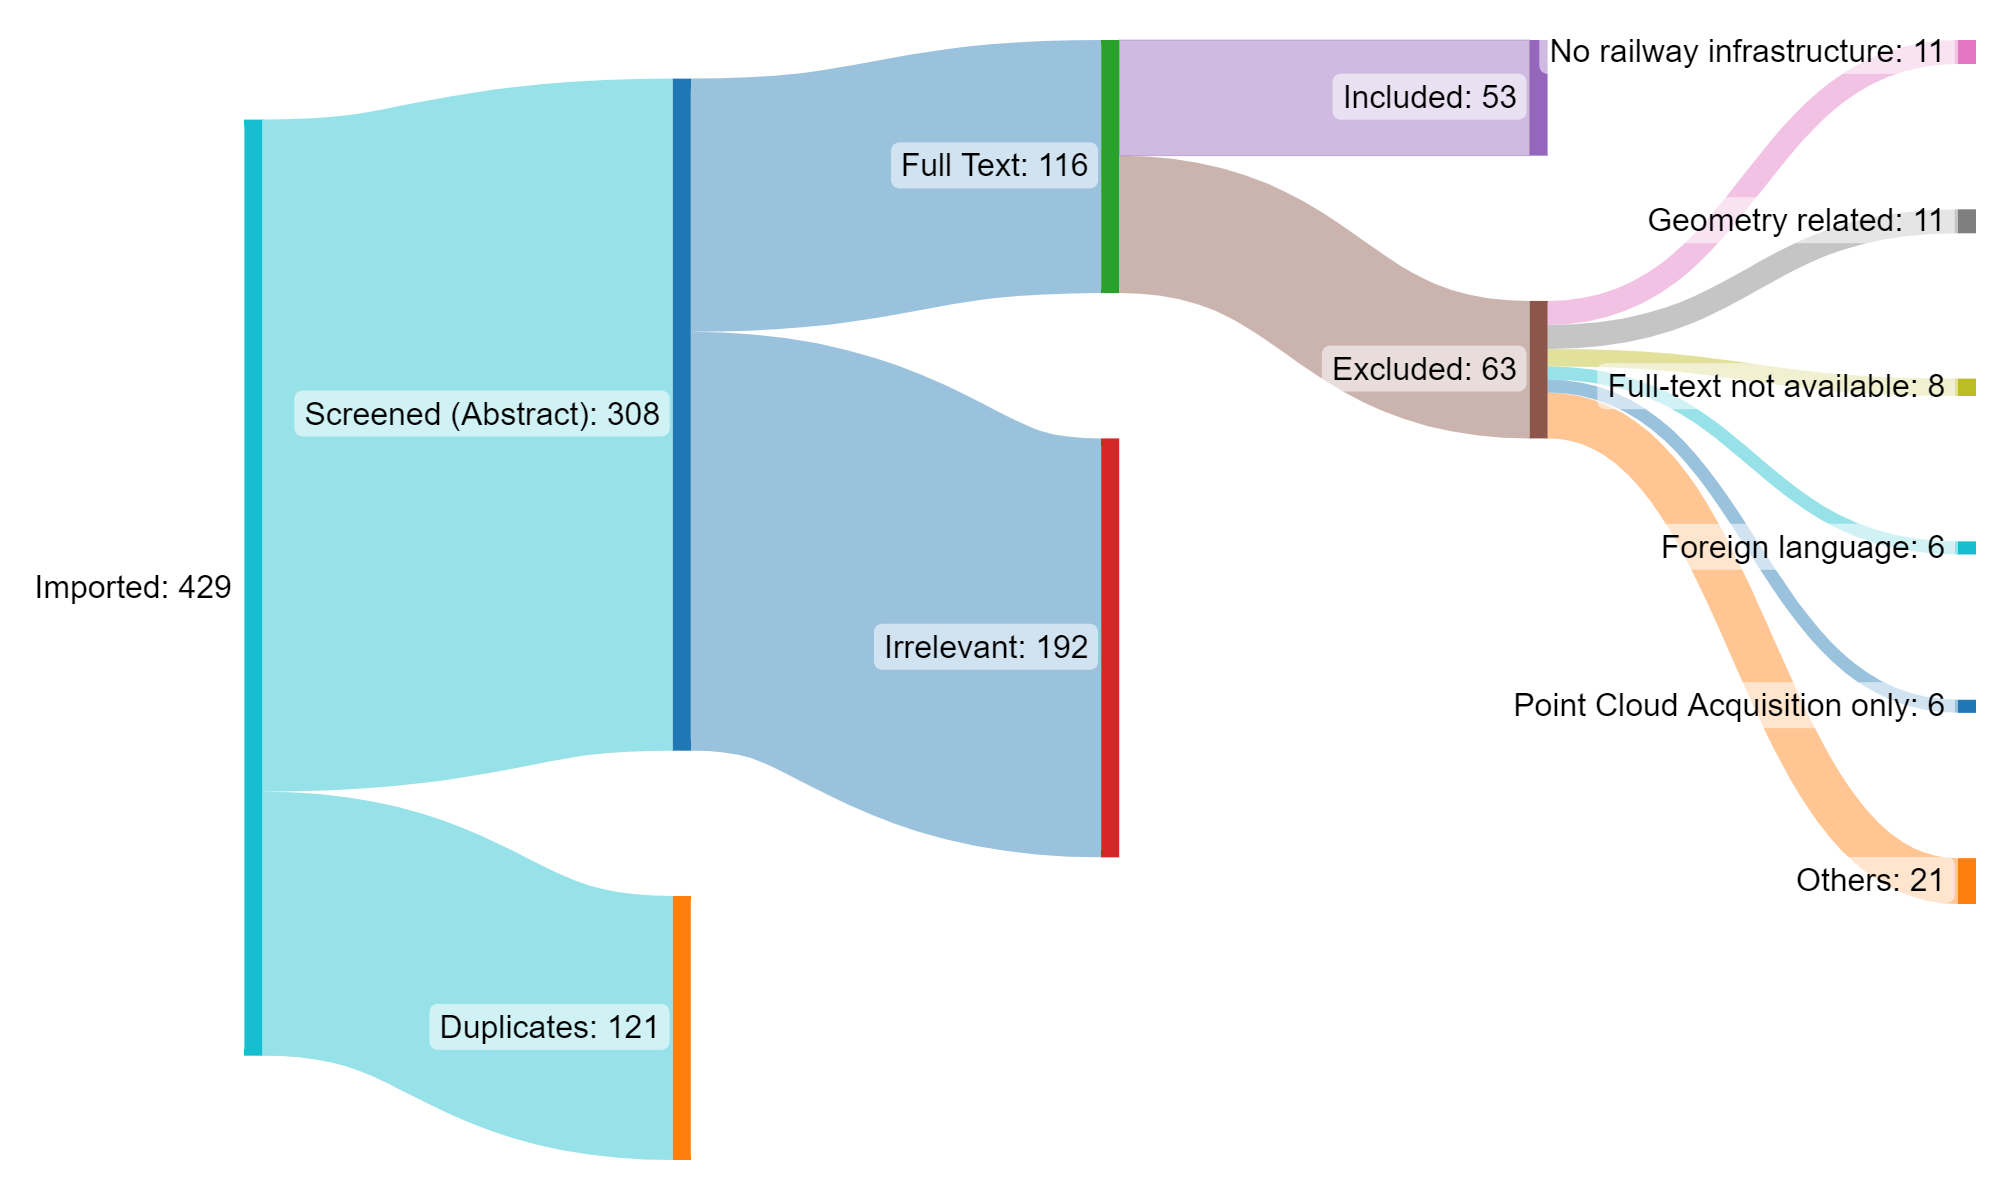
\includegraphics[width=0.95\linewidth]{./Chapters/stoa/fig/PrismaDiagram.png}
    \caption{An overview of the paper selection process with exclusion criteria.} 
    \label{fig:stoa:prisma}
\end{figure}

\subsection{Data extraction} % Extraction form used
In order to maintain the consistency of the data extraction process, we have used a form. The form is given in Table~\ref{tab:stoa:data-extraction}.
\begin{table}
    \centering
    \begin{tabular}{p{3.58cm}p{7.58cm}} %{|p{2.5cm}|p{8cm}|}
         \toprule
         \textbf{Field name} & \textbf{Description} \\
         \midrule
         Title & The title of the paper \\
         \addlinespace
         Goal & The main goal of the paper\\
         \addlinespace
         Steps & Which steps are described in the paper (pre-processing, modelling, digital twinning)? \\
         \addlinespace
         Pre-processing techniques & List the used pre-processing techniques \\
         \addlinespace
         Modelling techniques & List the used modelling techniques \\
         \addlinespace
         Digital twinning techniques & List the used digital twinning techniques \\
         \addlinespace
         Measurement of quality & What quality metrics are used? \\
         \addlinespace
         Country & From which country is the data in the dataset? \\
         \addlinespace
         Dataset & List characteristics of the dataset \\
         \addlinespace
         Experimental setup: speed & Speed of the vehicle while collecting the dataset\\
         \addlinespace
         Experimental setup: scanner type & Type of scanner used for collecting the dataset\\
         \addlinespace
         Experimental setup: RGB data & Are colours (or other additional information) present in the dataset?\\
         \addlinespace
         Notes & Any other relevant and interesting aspects\\
         \bottomrule
    \end{tabular}
    \caption{The data extraction form used for gathering useful information from every article.}
    \label{tab:stoa:data-extraction}
\end{table}
For the digitalisation of infrastructure, data collection plays a crucial role. Therefore, we have collected data reported in the selected studies related to data collection or meta-information. Most importantly, we collected the scan speed (speed of the vehicle if it is vehicle mounted), presence of colour information, or simultaneous collection of other sensory data such as GPS. Note that not all papers have described the data collection process. 

We divided infrastructure digitalisation into three stages. The first stage is pre-processing, where raw or filtered data is pre-processed for modelling purposes. The second stage is the modelling itself, while the last stage is the creation of digital twins. The `Steps' field is used to register which stages are described in the paper. The results section is also divided with respect to these stages.
The notes field is used to note down any other relevant information not covered by any other field. 
\section{Meta analysis, challenges, and datasets}\label{sec:stoa:metaanalysis}
To get a better insight into the gathered data, clusters of articles are formed based on common characteristics like publication year, nature of the dataset or analysis method used. 
It is apparent from Figure~\ref{fig:stoa:publication_over_year} that the point cloud analysis for railway scenes has been gaining interest in recent years. Another interesting observation is the dip in the number of publications for 2017--2019, with a further increase in 2020/2021. We cannot associate a reason to the dip in the number of publications. However, the increase can be attributed to the popularity of deep learning-based techniques. The rise in the utilization of deep learning techniques for point cloud data analysis can be significantly attributed to the seminal paper by \citeauthor{qi2017pointnet} in 2017, which introduces the PointNet model~\cite{qi2017pointnet}. This work was groundbreaking because it introduced a novel neural network that could process point clouds directly. Note that the data for the year 2022 is incomplete since the query was run in November 2022. 
\begin{figure}
    \centering
    \begin{tikzpicture}
        \begin{axis}[
            width=0.95\linewidth,
			height=0.625*0.95\linewidth,
        	axis x line*=bottom,
        	axis y line*=left,
        	ybar,
        	ymajorgrids=true,
        	ymin=0,
        	%enlargelimits=0.05,
        	bar width=15pt,
        	x tick label style={
        		/pgf/number format/1000 sep=,
        		rotate=45,
        		anchor=north east},
            %xlabel=Year,
        	ylabel=Count
        ]
        \addplot[sax-green,fill=sax-green] 
        	coordinates {
        	    (2011,2)
        	    (2012,1)
        	    (2013,2)
        	    (2014,2)
        	    (2015,3)
        	    (2016,7)
        	    (2017,3)
        	    (2018,1)
        	    (2019,4)
        	    (2020,11)
        	    (2021,11)
        	    (2022,6)
                };
        \end{axis}
    \end{tikzpicture}
    \caption{Number of publications per year (from papers included in this study)}
    \label{fig:stoa:publication_over_year}
\end{figure}

It was evident from the full-text search that most papers can be categorised into three classes based on the objective of the analysis. These steps were pre-processing, modelling, and digital twin. All papers have at least one of these aspects as the main contribution. The distribution of papers according to steps is given in Figure~\ref{fig:stoa:steps}. It is clear from the table that there is no single paper with digital twins as a core focus. In most cases, it is combined with modelling. A combination of pre-processing and modelling is understandably the most used.
\begin{figure}
    \centering
    \begin{tikzpicture}
        \begin{axis}[
            width=0.95\linewidth,
			height=0.625*0.95\linewidth,
        	axis x line*=bottom,
        	axis y line*=left,
        	ybar,
        	ymajorgrids=true,
        	ymin=0,
        	%enlargelimits=0.05,
        	bar width=15pt,
        	x tick label style={
        		%/pgf/number format/1000 sep=,
        		rotate=45,
        		anchor=north east},
          xtick={0,1,2,3,4},
          xticklabels={\textit{(PP,M)},\textit{M},\textit{(PP,M,DT)},\textit{(M,DT)},\textit{PP}},
            %xlabel=Year,
        	ylabel=Count
        ]
        \addplot[sax-green,fill=sax-green] 
        	coordinates {
        	    (0,25)
        	    (1,14)
        	    (2,9)
        	    (3,5)
        	    (4,3)
                  };
        \end{axis}
    \end{tikzpicture}
    \caption{An overview of the count of publication describing pre-processing(PP), modelling(M), and digital twin (DT). Note that there is no paper with a sole focus on digital twin.}
    \label{fig:stoa:steps}
\end{figure}


\subsection{Datasets} 
One interesting finding of our literature review is the lack of public benchmark datasets consisting of point clouds in the context of railway infrastructure. However, we have recently published a fully labelled dataset consisting of catenary arches~\cite{ton2022semantic}, which is the only openly available dataset to the best of our knowledge. Although a few datasets are mentioned in the literature, they are not openly accessible. 
The only paper we found concerning data collection in the context of railway infrastructure is \cite{sturari2017robotic} that have reported the most detailed data collection methodology. The authors have presented the approach together with pre-processing. The primary focus was on change detection for the safety and security of railway infrastructure~\cite{sturari2017robotic}. 

The datasets from the included studies are summarised in Table~\ref{tab:stoa:datasets}. The table presents a total of 46 datasets from diverse geographical locations, predominantly from China (11), the European Union (24), and other countries (11), showcasing global research interest. Various data acquisition methods are employed across studies. The majority of the studies used MLS (31), followed by ALS (8), TLS (3) and other methods (4). The datasets vary largely in terms of point density, ranging from densities as low as 50~points/$m^2$ to as high as 2500~points/$m^2$, and cover short stretches (80~m) to several kilometres (120~km). Additionally, while many studies focus on geometric data, only the minority of the datasets incorporate RGB information, highlighting the multifaceted nature of the research.

In the process of collating data for the table, we occasionally derived the density or length values from other information provided within the papers. A notable observation was the complete absence of publicly available datasets. While many papers emphasised the significance of point density, it was interesting to see that a quantitative report on density was often omitted rather it was described qualitatively like low or high density. Interestingly, there was a dataset that focused on lab-generated data of bolts~\cite{lu2021bolt}, but we chose to exclude it from the table for clarity. A particularly remarkable dataset~\cite{zhang2016automatic}, originated from China. Despite being recorded at an impressive speed of 193~km/h, it boasted an exceptionally high point density of 3000~points/$m^2$, underscoring the advancements in data acquisition techniques. For some datasets, we assumed that they were the same because they are from the same research group and have the same characteristics, although it was not stated explicitly in the papers.
%\begin{table}
%   \centering
\setlength{\tabcolsep}{2pt}
    \begin{ctabular}{p{2cm}p{2.5cm}p{2cm}p{1.5cm}p{1.5cm}p{1.5cm}p{1cm}}
        \toprule
        \textbf{Ref.} & \textbf{Country} & \textbf{Scanner type} & \textbf{Speed (km/h)} & \textbf{Density (p/m$^2$)} & \textbf{Length (m)} & \textbf{RGB} \\\midrule
        \cite{beger2011data}                                    & Austria & ALS & - & 60-90 & 120~000 & Yes \\ % density is p/m^2
        \cite{arastounia2015automated}                          & Austria & MLS & 125 & - & 550 & Yes \\
        \cite{oudeelberink2013rail}                             & Austria & MLS & - & 700 & 600 & No \\
        \cite{geng2020comparison}                               & China & ALS & - & - & - & No \\
        \cite{chen2020deep}                                     & China & MLS & 3.6 & - & 16~700 & No \\
        \cite{chen2021railway}                                  & China & MLS & - & - & 150 & No \\
        \cite{li2018methodology}                                & China & MLS & 120 & - & 3500 & No \\
        \cite{lin2020lidar,liu2021an,tu2020lidar}               & China & MLS & 3.6 & 1028 & 16.000 & No \\
        \cite{yu2022real-time}                                  & China & MLS & - & - & - & No \\
        \cite{zhang2016automatic}                               & China & MLS & 193 & 3000 & 11~690 & No \\
        \cite{xu2021vehicle-born}                               & China & MLS & 60 & - & 100~000 & No \\
        \cite{zou2019efficient}                                 & China & MLS & - & 490 & - & No \\
        \cite{cheng2019automatic}                               & China & TLS & - & - & 885 & No \\
        \cite{cui2020real-time}                                 & China & - & - & - & 2000 & No \\ % test set, training is only fasteners
        \cite{roberts2017monitoring}                            & England & MLS & - & - & 16~100 & No \\
        \cite{soilan20213D}                                     & Europe & - & - & - & 90~000 & No \\
        \cite{zhu2014the}                                       & Finland & ALS & - & 50 & 2000 & No \\ % They used orthophoto with color as additional data source but color is not directly in point cloud
        \cite{zhu2014the}                                       & Finland & MLS & 35 & 720 & 2000 & No \\
        \cite{manier2022railway}                                & France & ALS & - & - & 5250 & No \\
        \cite{mathani2022enhancing}                             & France & MLS & - & - & - & Yes \\
        \cite{manier2022railway}                                & France & MLS & - & - & 13~000 & No \\
        \cite{chbeir2015detection}                              & Germany & MLS & & & 50~000 & No \\
        \cite{karmacharya2015knowledge}                         & Germany & MLS & - & - & - & No \\
        \cite{ponciano2015detection}                            & Germany & MLS & - & - & 51~000 & No \\
        \cite{benhmida2011from,hmida2012knowledge-driven,truong2013automatic} & Germany & TLS & - & - & 500 & No\\
        \cite{wang2022farnet}                                   & Hong Kong & MLS & - & - & 16~000 & No \\
        \cite{cserep2022effective}                              & Hungary & MLS & 60 & - & 34~000 & Yes \\ % point density could be calculated (782p/m^2)
        \cite{sahebdivani2020rail}                              & Iran & Aerial \mbox{images} & - & - & 200 & Yes \\
        \cite{dibari2021semantic}                               & Italy & Stereo vision & - & - & 300 & Yes \\
        \cite{corongiu2020classification}                       & Italy & ALS & - & - & 1000 & No \\
        \cite{sturari2017robotic}                               & Italy & MLS & 0.36-3.6 & - & - & Yes \\
        \cite{Karunathilake20}                                  & Japan & MLS & 20 & 1600 & - & No \\
        \cite{arastounia2017enhanced,arastounia2016application} & Netherlands & ALS & 75 & - & 80 & No\\ % density per class
        \cite{ariyachandra2020detection,ariyachandra2020digital}& Netherlands & ALS & - & 293 & 18~000 & No\\ % density is p/m^2
        \cite{arastounia2017enhanced}                           & Netherlands & TLS & - & - & 630 & No \\% density per class
        \cite{kwoczynska2016elaboration}                        & Poland & ALS & - & 10-17 & 772 & No \\
        \cite{kwoczynska2016elaboration}                        & Poland & MLS & - & - & 550 & No \\
        \cite{pastucha2016catenary}                             & Poland & MLS & - & - & 90~000 & No \\
        \cite{gazero2019automated}                              & Portugal & MLS & - & - & 550 & No \\
        \cite{jung2016multi-range}                              & South Korea & MLS & 50-70 & 100-800 & 1000 & No \\
        \cite{jwa2015kalman}                                    & South Korea & MLS & 60 & 85 & 100 & No \\
        \cite{grandio2022point,lamas2021automatic,soilan2021fully} & Spain & MLS & 10 & 980 & 90~000 & No \\
        \cite{gutirrezfernndez2020automatic}                    & Spain & MLS & 4 & 2500 & - & No \\
        \cite{uggla2021towards}                                 & Sweden & MLS & - & 568 & 2000 & No \\ % length is avg width (33m) times # crossings (60), density is calculated from avg data
        \cite{marwati2021automatic}                             & Taiwan & MLS & - & - & 14~000 & No \\
        \cite{yang2014automated}                                & USA & MLS & - & 77 & 2000 & No \\
        \bottomrule
    \end{ctabular}
	\freetabcaption{An overview of the datasets used in the included papers.}\label{tab:stoa:datasets}
	\setlength{\tabcolsep}{6pt} % Restore
 %   \caption{An overview of the datasets used in the included papers.}
 %   \label{tab:stoa:datasets}
%\end{table}

\subsection{Challenges of point cloud data}\label{sec:stoa:differences_challenges_pc_data}
Point clouds are irregular, unstructured and unordered, unlike 2D images, and are thus a challenging data type to work with~\cite{bello2020deep}. Following is a list of the most significant challenging characteristics that are inherent to point cloud data. Sensor type, environment, weather conditions, and sensing distance influence the degree to which point clouds suffer from these characteristics~\cite{li2020deep}:

\begin{description}
    \item[Irregularity] point clouds usually have non-uniform distributed point density. 
    \item[Unstructured] point clouds are not placed on a regular grid. Each point is scanned independently, and its distance to neighbouring points is not fixed. This also means that voxelisation of point clouds often leads to empty voxels, i.e. data sparsity.
    \item[Unordered] point clouds are sets of points, the order in which the points are stored does not change the representation. 
    \item[Size] point clouds often contain millions of points taking up large chunks of memory and thus it is time-consuming to process and analyse them.
    \item[Measurement artefacts] point clouds can contain noise in the data produced for example by errors of the scanner or moving objects~\cite{nurunnabi2015outlier}.
    \item[(Partial) Occlusion] point clouds suffer from (partial) occlusion of objects since other objects may block them~\cite{guo2015novel}.
\end{description}

A challenge for railway scenes is the large variance in object sizes (a top bar can be well over 20~metres long, while an insulator typically is around 30~centimetres~\cite{ton2022semantic}, which is a size ratio of at least 60 times). An additional challenge is the huge class imbalance encountered within the rail environment, for instance certain objects like masts occur very regularly, but relay cabinets occur a lot less often.
\section{Pre-processing}\label{sec:stoa:preprocessing}
Point clouds are unordered sets of points. Absence of structure makes them a challenging datatype to deal with. Pre-processing techniques help to reduce the volume of data, introduce a structure or filter out the dispensable points. In certain cases the boundary between pre-processing and modelling is blurred due to the fact that the result of pre-processing is sometimes already a feature. Therefore, we do not apply the term in their strict sense instead focus on the mechanisms of the techniques. 

In general, the main goal of the pre-processing is to cull points such that further processing steps require less computational effort. In the following subsections we list the pre-processing techniques found in literature and their associated references.

\subsection{Cropping}
Cropping is a very rudimentary pre-processing step that removes points based on a specified bounding region. This is predicated on the assumption that the points outside this region do not contain information of interest. For instance, the work of \citeauthor{ariyachandra2020digital}, which focuses on detecting elements of the overhead line equipment, remove all points belonging to the ground by setting a threshold value of 0.23~cm. Points with a $z$-coordinate below this threshold are removed~\cite{ariyachandra2020digital}. Similarly \citeauthor{chen2020deep} also use fixed thresholds to remove distant points with no information~\cite{chen2020deep}. A more advanced method of detecting ground points is proposed by \citeauthor{chen2021railway} which use a Euclidean distance clustering segmentation algorithm~\cite{chen2021railway}. When point clouds are collected using a mobile scanner mounted on a train, the trajectory log can play an important role in the culling of points. As an example, Pastucha defines an extent of 5~m on both sides of the trajectory. Points outside of this region are removed. The scan angle, which is usually recorded as meta-data of a point, can also be used as a filter condition to remove points~\cite{gazero2019automated}. As an example of how the scan angle can be used to crop relevant regions of points, the authors show how the track centre lines and the ballast top can easily be recognised from the point cloud data.
To remove vegetation, the work of \citeauthor{cserep2022effective} first project the scene to 2D by registering the maximum value of the \(z\)-coordinate. After this contour detection is used to filter out vegetation~\cite{cserep2022effective}, unfortunately no further details are provided for this approach.

Which points to cull is also highly dependent on the application. If the application is to detect tracks, it makes sense to only maintain points which relate to the tracks. Specifically for this purpose, \citeauthor{ponciano2015detection} use a mask-based approach to only keep points which relate to the tracks~\cite{ponciano2015detection}. An alternative approach provided by \citeauthor{zou2019efficient} first filter the point cloud based on intensity values, only values with a low intensity are kept. After filtering, tracks remain, but still there is significant noise. Further refinement steps are required to extract the tracks~\cite{zou2019efficient}.

\subsection{Partitioning}
Commonly the point cloud data provided covers a large area. In order to create tractable pieces that can be used in downstream processing steps the larger point cloud is usually partitioned into smaller pieces. \citeauthor{ariyachandra2020digital} manually partitioned a large point cloud that covered \(\approx\)18~km into three pieces covering \(\approx\)6~km each~\cite{ariyachandra2020digital}. In a related work, the same authors employed an optimisation strategy to determine the optimal number of partitions for splitting the dataset~\cite{ariyachandra2020detection}. Constraints used in this optimisation approach were the curvature of the track, number of noise points, and the cropping of masts. The width of the scenes was limited to 30~m.

The work of \citeauthor{lamas2021automatic} use the trajectory log of the measurement train to partition the data into pieces which are 100~m long and 20~m wide~\cite{lamas2021automatic}. Pastucha uses even smaller sections which are 0.5~m in length~\cite{pastucha2016catenary}. Surprisingly, only a limited number of studies utilise the raw frame-by-frame data from scanner, with most relying solely on aggregated results. An exception is the work of \citeauthor{chen2020deep} that use 2D laser scan lines to segment the overhead contact system~\cite{chen2020deep}. This raw frame data is commonly used for applications such as autonomous driving. The envisioned benefit of using this raw data is that the data will have a fixed frame of reference, i.e. it is always known how the data is captured with reference to the current track.

\subsection{Normalisation}
Normalisation of the training data plays an important role, especially when deep learning methods are involved. To align individual pieces of point cloud data along the $x$-axis \citeauthor{ariyachandra2020detection} use a Principle Component Analysis (PCA) to determine the major axis of the point cloud~\cite{ariyachandra2020detection}. The work of \citeauthor{lamas2021automatic} also use PCA, albeit in a slightly modified form, to align the direction of the tracks along the $x$-axis. \citeauthor{corongiu2020classification} align the point cloud subsets to the $y$-axis, unfortunately the method to do so is not described~\cite{corongiu2020classification}. The trajectory log of the mobile sensing platform facilitates a convenient way of aligning sub-point cloud to the track~\cite{pastucha2016catenary}. Of course, the aforementioned partitioning of the scene into regular-sized pieces is also a form of normalisation.

\subsection{Projection}
As point cloud data has no structure, sometimes the point cloud is projected to a 2D plane with a grid to create an image. This image can then be processed with conventional image processing techniques. For example, \citeauthor{corongiu2020classification} flatten the point cloud to a 2D grid by summing in the $z$-direction. Within this image masts will be visible as high-intensity blobs, making it easy to locate them~\cite{corongiu2020classification}.
\par An interesting piece of work, albeit in a very premature state, is presented by \citeauthor{wolf2021asset} Their approach to detect railway assets from point cloud data is to first render a greyscale image from a slice of point cloud data~\cite{wolf2021asset}. The pixel values are the intensity values from the original point cloud data. These slices are taken perpendicular to the rail track. The work shows results of both object detection, based on the YOLOv3 model~\cite{yolov3}, and on semantic segmentation, based on U-Net~\cite{unet}. An image-based approach has two major benefits: the field of image processing has advanced much further than point-based methods and the processing of raster data can be done much more efficiently compared to point data.

\subsection{Data structures}
Voxelisation is the process of defining a regular 3D grid, each element of the grid is referred to as a voxel. This is analogous to a pixel in the 2D case. The benefit of the voxelisation process is that it creates a structured format which can be processed very efficiently. For example, \citeauthor{jung2016multi-range} extract line segments per voxel~\cite{jung2016multi-range}. Another data structure which occurs is the \textit{kd}-tree, this data structure is used for efficiently selecting neighbour points around a query point~\cite{arastounia2015automated}.

When point clouds are captured using a laser scanner, the captured point density close to the sensor is higher compared to regions further away from the sensor. To homogenise the density across the entire scene, a fixed number of points per voxel can be retained~\cite{lamas2021automatic,grandio2022point}. Not only does this improve the homogeneity of the point distribution, but it also reduces the number of points.


Besides voxelisation, different grid definition schemes are possible. For instance, \citeauthor{yu2022real-time} use pyramid partitions~\cite{yu2022real-time}. This approach defines smaller volumes close to the sensor and increases the volume gradually when the distance to the sensor increases. This ensures that the number of points per volume remains roughly the same.

\subsection{Sampling}
Down-sampling is a common pre-processing step to reduce the number of points or to achieve a fixed number of points~\cite{cui2020real-time, grandio2022point}. Fixed number of points are usually required when training deep learning models. For instance, \citeauthor{grandio2022point} used a fixed size of 16384 (\(2^{14}\)) and 32768 (\(2^{15}\)) points for training a \pnpp{} segmentation model~\cite{grandio2022point}. Note that it is a common misconception that such models \textit{require} a fixed number of points as input. The architecture of these models are agnostic of the point set size, but the frameworks used to implement the models are the bottleneck.

To create tractable pieces which can be used during training of a deep learning model, \citeauthor{grandio2022point} extract cubes with a fixed edge length of 10~$m$ from larger scene~\cite{grandio2022point}. The work of \citeauthor{corongiu2020classification} extract a cylindrical region (radius=$2~m$) of interest around candidate points. These cylindrical regions are then further processed to create a semantic segmentation~\cite{corongiu2020classification} of the scene.

Using information from the scanning geometry and the time-stamp metadata of each point it is possible to extract consecutive cross sections of the railway bed area~\cite{yang2014automated}. These so-called scan lines are then further processed to extract the track locations.

\subsection{Feature extraction}
Point clouds offer a rich source of data from which a plethora of features can be derived. Geometrically, one can extract attributes such as normal vectors and curvature. From a statistical perspective, features like local density and variance are valuable. In terms of shape, roughness and linearity provide insights into the structure of the data. Topologically, connectivity sheds light on the relationships between data points. Additionally, when colour information is available, RGB values can be harnessed. These extracted features, encompassing geometric, statistical, shape, topological, and colour attributes, serve as foundational elements for subsequent modelling endeavours.

\citeauthor{geng2020comparison} provide a comparison of several feature extraction methods applied to a point cloud scene of a Chinese high-speed railway collected using an airborne laser scanner~\cite{geng2020comparison}. The work of \citeauthor{jung2016multi-range} extract line segments per voxel~\cite{jung2016multi-range}. These line segments are then classified using a multi-range Conditional Random Field (CRF) classifier.

\subsection{Others}
The majority of the works use laser scanning techniques to capture a point cloud. An alternative approach is to use photogrammetry techniques to create a point cloud based on image data. This is done in the work of \citeauthor{sahebdivani2020rail} which use a commercial drone to capture images from the area of interest. These images are then processed to create a point cloud~\cite{sahebdivani2020rail}. The use of structured light is another approach to create point clouds, this is done by \citeauthor{cui2020real-time} in their work to automatically inspect railway fasteners~\cite{cui2020real-time}. 

One pre-processing step which is often lacking from literature is the processing of the raw point cloud data. Often laser scanners will produce a stream of frames. These frames are then combined to create a larger point cloud scene. During this processing step, the points are also mapped from their sensor's local reference frame to a global coordinate reference system. To do so, an accurate Global Navigation Satellite System (GNSS) is required. The reception and accuracy of GNSS is not always consistent, therefore GNSS data is often augmented with gyroscope, heading and odometer data. The work of \citeauthor{xu2021vehicle-born} sheds some light on this matter~\cite{xu2021vehicle-born}. During the processing of raw frames into larger scenes, also duplicate measurements are excluded. For instance, when the measurement train is standing still, data is still being collected. This will contain a lot of redundant data, which is removed during post-processing.

\subsection{Summary of pre-processing techniques}
The pre-processing techniques described above are tied closely to the purpose and each of them has its advantages and challenges. The choice of the techniques is mostly dependent on the context and the data. In Table~\ref{tab:stoa:pre-processing}, we provide a concise summary and comparison of these techniques. We have also included their use in the context of railway infrastructure as a result of our literature study. From the table, it is evident that these pre-processing techniques are not mutually exclusive. Instead, several techniques are often employed to maximise their collective benefit. 

\begin{table}[!ht]
\centering
\begin{tabular}{%
l%
>{\raggedright\arraybackslash}p{3cm}%
>{\raggedright\arraybackslash}p{3cm}%
>{\raggedright\arraybackslash}p{2cm}}\toprule
\textbf{Technique} & \textbf{Challenges} & \textbf{Advantages} & \textbf{References}\\
\midrule
Cropping &
\textbullet\,Determining optimal boundaries.
\textbullet\,Potential loss of important data.& 
\textbullet\,Reduces data size for faster processing. 
\textbullet\,Focuses on regions of interest. & \cite{ariyachandra2020digital,chen2020deep,gazero2019automated,ponciano2015detection,zou2019efficient}\\
\addlinespace
Partitioning & 
\textbullet\,Deciding optimal partition size. 
\textbullet\,Handling boundary data between partitions. & 
\textbullet\,Manages large datasets by breaking them into manageable chunks. & \cite{ariyachandra2020digital,ariyachandra2020detection,lamas2021automatic,chen2020deep}\\
\addlinespace
Normalisation & 
\textbullet\,Determining appropriate scale. 
\textbullet\,Potential loss of original data characteristics. & 
\textbullet\,Standardises data range. 
\textbullet\,Enhances compatibility with algorithms requiring normalised data. &\cite{ariyachandra2020detection,corongiu2020classification,pastucha2016catenary} \\
\addlinespace
Projection & 
\textbullet\,Loss of 3D information. 
\textbullet\,Deciding optimal projection plane. & 
\textbullet\,Converts 3D data to 2D for easier visualisation and processing. & \cite{corongiu2020classification,wolf2021asset}\\
\addlinespace
Data Structures & 
\textbullet\,Complexity in implementation. 
\textbullet\,Overhead in memory and computation. & 
\textbullet\,Efficient data access and manipulation. 
\textbullet\,Supports advanced algorithms and operations. & \cite{jung2016multi-range,arastounia2015automated,lamas2021automatic,grandio2022point,yu2022real-time}\\
\addlinespace
Sampling & 
\textbullet\,Potential loss of detail. 
\textbullet\,Choosing appropriate sampling method and density. & 
\textbullet\,Reduces data size.
\textbullet\,Speeds up processing. & \cite{cui2020real-time,grandio2022point,grandio2022point,corongiu2020classification,yang2014automated}\\
\addlinespace
Feature Extraction & 
\textbullet\,Deciding relevant features. 
\textbullet\,Complexity in feature computation. & 
\textbullet\,Reduces data dimensionality. 
\textbullet\,Enhances data characteristics for specific tasks. & \cite{geng2020comparison,jung2016multi-range} \\
\bottomrule
\end{tabular}
\caption{Comparison of pre-processing techniques for point clouds and their use in the context of railway infrastructure.}\label{tab:stoa:pre-processing}
\end{table}
\section{Modelling techniques} \label{sec:stoa:modelling}
In this section, we compile a glossary of methods, algorithms, and techniques for modelling point clouds, designed for purposes like object classification, segmentation, and object detection. We categorise and describe these methods found in the literature, focusing on their strengths and limitations. The point cloud modelling methods are broadly divided into two categories: structure-based methods and machine learning-based methods. We describe each of these and their sub-categorisation. 
Two aspects are linked to modelling. One is the performance metric, while the other is the type of railway infrastructure being modelled. We start this section by providing information on these two essential aspects. 

%%%%%%%%%%%%%%%%%%%%%%%
\subsection{Rail infrastructure}
An essential aspect to consider in the railway environment is the modelling goal concerning railway infrastructure. While several researchers have focused on specific components of the infrastructure, the complete railway infrastructure is often overlooked.  In Table~\ref{tab:stoa:rail_infra} we have summarised the most commonly studied infrastructure components along with the corresponding research references.
\par It is important to acknowledge that certain aspects of the railway infrastructure, such as foreign objects, bridges, and tunnel deformation, have not been included in this paper due to the set exclusion criteria. Nevertheless, these areas have been gaining interest, particularly in the context of predictive maintenance and the expansion of high-speed rail networks in China (e.g., \cite{chen2021railway}). As the railway industry continues to evolve, exploring these aspects becomes increasingly crucial for comprehensive railway infrastructure modelling and analysis.
\begin{table}[!ht]
    \centering
    \begin{tabular}{ll}\toprule
       \textbf{Rail Component}  & \textbf{Reference}\\\midrule
        Rail Track detection and classification & \cite{arastounia2016application,cui2020real-time}\\
        Cable detection and classification & \cite{arastounia2016application,ariyachandra2020digital,corongiu2020classification,gutirrezfernndez2020automatic}\\
        Switch and crossing detection & \cite{chbeir2015detection,benhmida2011from,hmida2012knowledge-driven,ponciano2015detection}\\\bottomrule
    \end{tabular}
    \caption{Break down of the literature based on railway component.} \label{tab:stoa:rail_infra}   
\end{table}

\subsection{Performance metrics}
To evaluate the performance of modelling techniques various metrics can be used. In the following, We define the most popular metrics used in the context of point clouds. 
\subsubsection{Accuracy, Precision, Recall, $F_1$-score}
These are commonly used metrics for evaluating classification accuracy. For the sake of completeness they are defined below:
\begin{itemize}
\item \textbf{Accuracy} measures the overall correctness of a model's predictions by calculating the ratio of correctly predicted instances to the total number of instances (Equation~\ref{eq:stoa:acc}). It provides a general assessment of how well the model performs across all classes. The formula for accuracy is:
\begin{equation}
    Accuracy = \frac{TP+TN}{TP+TN+FP+FN}
    \label{eq:stoa:acc}
\end{equation}
where $TP$ stands for true positive, $TN$ is the true negative, $FP$ is false positive, and $FN$ is the false negative. 
\item \textbf{Precision} focuses on the proportion of correctly predicted positive instances out of all instances predicted as positive (Equation~\ref{eq:stoa:prec}). It provides insight into the model's ability to avoid false positives (instances predicted as positive but are actually negative). The formula for precision is:
\begin{equation}
    Precision = \frac{TP}{TP + FP}
    \label{eq:stoa:prec}
\end{equation}
\item
\textbf{Recall}, also known as sensitivity or true positive rate, measures the proportion of correctly predicted positive instances out of all actual positive instances (Equation~\ref{eq:stoa:rec}). It indicates the model's ability to identify all positive instances and avoid false negatives (instances predicted as negative but are actually positive). The formula for recall is:
\begin{equation}
    Recall = \frac{TP}{TP + FN}
    \label{eq:stoa:rec}
\end{equation}
\item
The $\mathbf{F_1}$\textbf{-score} is a harmonic mean of precision and recall (Equation~\ref{eq:stoa:f1}). It provides a balanced measure that takes into account both precision and recall. The $F_1$-score is useful when one want to consider both false positives and false negatives equally. The formula for the $F_1$-score is:
\begin{equation}
    F_1\text{-}score = 2\frac{ Precision \cdot Recall}{Precision + Recall}
    \label{eq:stoa:f1}
\end{equation}
In the case of Boolean data, the $F_1$ score is also sometimes referred to as the S\o rensen-Dice coefficient.
\end{itemize}


\subsubsection{Root Mean Square Error (RMSE)}
It is the standard deviation of prediction error (Equation~\ref{eq:stoa:rmse}). It is often used for regression problems. The formula to compute RMSE is:
\begin{equation}
    \mathit{RMSE}=\sqrt{\frac{\sum_{i=1}^N(Actual_i-Predicted_i)^2}{N}}
    \label{eq:stoa:rmse}
\end{equation}

\subsubsection{Mean Intersection over Union}
Mean Intersection over Union (mean IoU) is a metric commonly used in evaluating the performance of semantic segmentation models. It measures the overlap between the predicted segmentation and the ground truth segmentation.

The Intersection over Union (IoU), also known as Jaccard Index, for a single class is calculated by dividing the size of the intersection of pixels between the predicted and ground truth masks by the size of the union of those pixels (Equation~\ref{eq:stoa:iou}). It provides a measure of how well the model accurately captures the boundaries and regions of the objects of interest.

The mean IoU is then computed by averaging the IoU values across all classes or categories. It provides an overall assessment of the segmentation model's performance, taking into account the accuracy of segmenting multiple classes simultaneously.

The formula for calculating IoU is:
\begin{equation}
    IoU = \frac{|\text{$Predicted$ $mask$ $\cap$ $ground$ $truth$ $mask$}|}{|\text{$Predicted$ $mask$ $\cup$ $ground$ $truth$ $mask$}|}
    \label{eq:stoa:iou}
\end{equation}

Where $\cap$ is the intersection, $\cup$ is the union and $|\,\cdot\,|$ is the cardinality.
The mean IoU is computed by taking the average IoU across all classes or categories (Equation~\ref{eq:stoa:miou}). Here, $N$ is the total number of classes:
\begin{equation}
    \text{Mean IoU} = \frac{1}{N}\sum_{i=1}^N \text{IoU class } i
    \label{eq:stoa:miou}
\end{equation}

Mean IoU values range from 0 to 1, with 1 indicating a perfect overlap between the predicted and ground truth masks, and 0 indicating no overlap at all. Higher mean IoU values indicate better segmentation performance.

\subsection{Structure-based methods}\label{subsec:stoa:structure based methods}
Structure-based methods exploit or enforce structure to the point cloud scenes. These methods utilise the geometric and topological properties of point clouds and often rely on mathematical models to extract meaningful information from the point cloud data. 

These methods leverage geometric and topological properties, enabling them to represent the underlying 3D structure and surfaces accurately. Moreover, these methods are frequently characterised by well-defined mathematical models. These models not only enhance our understanding of the underlying processes but also ensure precision during implementation.

Besides their advantages the structure-based methods have limitations too. The methods could struggle to model surfaces that are complex since the underlying principles rely on basic geometric primitives. Additionally, they can handle noise to a certain level but remain sensitive to a high noise level and outliers that can impact their performance and limit their usability. Moreover, structure-based methods could be computationally intense and they do not profit from higher point densities. Their lack of adaptability is another drawback, as they are often tailored to specific application domains and may not generalise well to diverse datasets.  

These methods can be further categorised (see e.g.~\cite{grilli_review_2017,nguyen_3d_2013}). The following subsections describe these sub-categories and their use in the context of the railway environment. 

\subsubsection{Edge-based methods}
Edge-based methods usually have two main stages: (i) detecting edges to outline borders of different regions followed by (ii) the grouping of points inside boundaries to generate the final segments. Edges are defined by points where changes in the local surface properties exceed a given threshold. Local surface properties are for instance normals, gradients, principal curvatures or higher-order derivatives. Edge-based methods are generally fast but may produce inaccurate results in case of noise and uneven density of point clouds. When disconnected edges are detected, a filling or interpretation procedure is applied to identify closed segments.
\citeauthor{ariyachandra2020detection} \cite{ariyachandra2020detection} used this method to detect pole-like objects. Their approach was based on line detection and point clustering. 

\subsubsection{Region-growing methods}
Region-growing methods start from one or more seed points that possess specific characteristics and then expand to neighbouring points with similar characteristics. These characteristics are for example surface orientation, curvature, etc. Bottom-up approaches start from some seed points and grow the segments on the basis of given similarity criteria. Bottom-up region-growing algorithms include two steps: identification of the seed points and adding points to them based on predefined criteria. Top-down approaches start by assigning all points to one segment and then subdivide the segment into smaller ones guided by certain thresholds. Region-growing methods are robust to noise (see e.g. \cite{lu2021supervoxel}), but they are sensitive to (i) the location of initial seed regions and (ii) inaccurate estimations of the normals and curvatures of points near region boundaries. For an explicit description of the region-growing algorithm in the context of railways, the interested reader is referred to~\citeauthor{cserep2022effective} \cite[Algorithm~1 and Algorithm~2]{cserep2022effective}.
Other examples of region-growing algorithms can be found in the work of \citeauthor{arastounia2017enhanced} \cite{arastounia2017enhanced}, \citeauthor{chbeir2015detection} \cite{chbeir2015detection}, 
\citeauthor{zhang2016automatic} \cite{zhang2016automatic}, \citeauthor{lu2021bolt} \cite{lu2021bolt}, and \citeauthor{zou2019efficient} \cite{zou2019efficient}. 

\subsubsection{Model fitting methods}
Model fitting methods are based on the observation that a lot of objects are built-up out of geometric primitives like planes, cylinders and spheres. Primitive shapes are fitted onto the point cloud and the points that comply with the mathematical representation of the primitive shape are labelled as one segment. Widely employed algorithms for model fitting are Hough Transform (HT), Random Sample Consensus (RANSAC) and fast point feature histograms (FPFH). Note that HT and FPFH are used to generate features that are utilised as an input for the model fitting methods such as RANSAC~(see e.g.~\cite{li20233D}). Model fitting methods are fast and robust with outliers. However, they fall short when dealing with complex shapes or fully automated implementations. Moreover, they have problems when dealing with different scales of input point clouds.
References that utilise these techniques in the context of railways are 
\cite{arastounia2016application,ariyachandra2020digital,benhmida2011from,beger2011data,oudeelberink2013rail,pastucha2016catenary}. 
A comparison of these methods is presented in~\cite{cserep2022effective}.

\subsubsection{Graph-based methods}
Graph-based methods view point clouds as graphs. In the simplest model, the vertices in the graph correspond to points in the data and the edges represent certain pairs of neighbouring points~\cite{dgcnn19}. An alternative approach is to first aggregate points into coherent patches, these patches are then considered as the vertices of the graph~\cite{Landrieu18}. Other techniques first voxelise the cloud with for example an octree or supervoxel method and construct a graph out of the voxelised point cloud. Graph-based methods are able to segment complex scenes in point cloud data with noise or uneven density with good results for example by finding the minimum-cut of the graph. However, these methods usually can not run in real-time and some of them may need an offline training step. Although the technique is applied in other contexts it is not applied in the context of railway environments. 

\subsubsection{Hybrid methods}
Multiple different methods are combined to exploit the best parts of the methods. Most of the reviewed papers fall under this category. Examples include
\cite{arastounia2016application,ariyachandra2020detection,ariyachandra2020digital,chbeir2015detection,Karunathilake20}.
\citeauthor{zhang2016automatic} has used several algorithms to extract power lines. They used the spatial structure of the power line for initial segmentation followed by a region-growing method. They applied PCA on the results of the region-growing algorithm and as a final step, they used least square fitting algorithm to model power lines~\cite{zhang2016automatic}. 
\citeauthor{zou2019efficient} has used a combination of \textit{k}-mean clustering and region-growing algorithm to extract railway tracks from point cloud data. Their focus was on extracting railway tracks with complex topology like bends and turnouts~\cite{zou2019efficient}.

\subsubsection{Summary of structure-based methods}
\par All structure-based methods have their strong and weak points. 
In Table~\ref{tab:stoa:structure-based-compare}, we have tabulated the advantages and challenges associated with each of these methods. We have also included the use of these methods in the context of the railway environment based on our literature search. 

\begin{table}[!ht]
    \centering
    \begin{tabular}{%
	  >{\raggedright\arraybackslash}p{1.58cm}%
	  >{\raggedright\arraybackslash}p{3.58cm}%
	  >{\raggedright\arraybackslash}p{3.58cm}%
	  >{\raggedright\arraybackslash}p{1.58cm}}\toprule
    \textbf{Method}       & \textbf{Advantages}          & \textbf{Challenges} & \textbf{References} \\\midrule      
     Edge-based & 
     \textbullet\,Effective in detecting sharp features and boundaries
     \textbullet\,Useful for feature extraction and edge detection
    & 
    \textbullet\,Sensitive to noise and outliers
    \textbullet\,Limited in handling non-sharp transitions
    & \cite{ariyachandra2020detection}\\ \addlinespace
    
    Region growing & 
    \textbullet\,Generates coherent and connected regions
    \textbullet\,Robust to noise and capable of handling irregular shapes
    & 
    \textbullet\,Sensitivity to seed point selection
    \textbullet\,May struggle with complex structures
    & \cite{arastounia2017enhanced,chbeir2015detection,zhang2016automatic,zou2019efficient} \\ \addlinespace
    
    Model fitting & 
    \textbullet\,Provides accurate geometric representations
    \textbullet\,Useful for shape recognition and surface reconstruction
    & 
    \textbullet\,Prone to model selection bias
    \textbullet\,Computational complexity for complex models
    & \cite{arastounia2016application,ariyachandra2020digital,benhmida2011from} \\ \addlinespace
     
    Graph-based & 
    \textbullet\,Captures geometric relationships effectively
    \textbullet\,Suitable for segmentation, classification, and features
    & 
    \textbullet\,Complexity in designing and training GCNs
    \textbullet\,Requires graph construction and processing overhead
    &--\\ \addlinespace
    
    Hybrid & 
    \textbullet\,Combine strengths of multiple methods to leverage complementary information
    & 
    \textbullet\,Memory and computational overhead could be higher
    \textbullet\,Integration and hyperparameter tuning could be a challenge
    & \cite{arastounia2016application,ariyachandra2020detection,ariyachandra2020digital,chbeir2015detection,Karunathilake20,zhang2016automatic,zou2019efficient}\\\bottomrule
    \end{tabular}
    \caption{Comparison of structure-based methods for point clouds.\label{tab:stoa:structure-based-compare}}
\end{table}


\subsection{Machine learning-based techniques}
Machine learning algorithms owe their success to their ability to learn from data. The popularity and widespread adoption of these algorithms can be largely attributed to the vast availability of data. Unlike structural methods, machine learning approaches are inherently adaptive, autonomously discovering patterns in the data. The performance of machine learning methods heavily relies on the quantity and quality of the training data. 

Various machine learning techniques have been developed specifically tailored to the unique structure of point clouds. As mentioned before, working with point cloud data presents its challenges, and the degree of success achieved by these algorithms is often limited. Many of these algorithms struggle to generalise well to different domains. Unlike computer vision problems, where large pre-trained models are readily available for transfer learning, point cloud tasks lack such widespread pre-trained resources. Besides its limitation, the use of machine learning-based techniques is trending, which will become apparent in the following sections. The machine learning-based techniques can be broadly categorised as traditional machine learning-based techniques and deep learning techniques. 
%%%%%%%%%%%%%%%%%%%
\subsubsection{Traditional machine learning}
Traditional machine learning methods are employed as an evolution towards methods that learn from the data and have better generalisability. The main difference with deep learning methods is that deep learning methods learn the features themselves. This is generally faster and more efficient since the model can derive more complex features and can distinguish the most informative features. 
The literature on traditional machine learning in the context of the railway environment is currently limited. 

\citeauthor{sturari2017robotic} have presented a traditional machine learning approach. The primary focus was on data collection methodology, and to provide proof of concept for applicability of machine learning to the collected dataset. They have compared four traditional machine learning methods, namely decision tree, support vector machine, \textit{k}-nearest neighbour and random forest with a convolution neural network. Notice that the learning task differed since the authors were concerned with the classification problem instead of segmentation or object detection~\cite{sturari2017robotic}. 

The approach used by \citeauthor{uggla2021towards} is interesting since they combined synthetic and real-world data to create synthetic railway scenes. They compared the performance of the deep learning-based approach on real scenes and the scenes synthetically generated from a point cloud. They concluded that the synthetic data could be helpful in generalising performance since more data can be generated easily instead of going through a lengthy data collection process~\cite{uggla2021towards}. 

%%%%%%%%%%%%%%%%%%%%%%%%%%%
\subsubsection{Deep learning based methods}
The problem of point cloud segmentation and classification looks similar to the ones in computer vision. However, the segmentation and classification are much more challenging for point clouds due to the absence of the grid structure. In computer vision, the images are represented using a structured grid of pixels that allows the application of a convolution neural network (CNN) to extract features. This structure is not present in point clouds. Thus, CNN cannot be directly applied. 

The point clouds are irregular and sparse since the density and distribution of points can vary significantly between different scenes and objects. 
Deep learning on point clouds requires a distinct approach, and it is currently attracting increasing interest from researchers, particularly in the context of self-driving cars~\cite{li2020deep}. For an empirical comparison of various deep learning approaches, the interested reader is referred to~\cite{guo2020deep}. It is worth mentioning that~\citeauthor{guo2020deep} conducted an empirical comparison of existing deep learning-based approaches for 3D point clouds using various benchmark datasets. However, it is important to note that none of these benchmark datasets specifically include the railway environment. 

The deep learning-based methods can be broadly classified into three categories based on how they handle the point clouds. The categories, indirect methods, direct methods and hybrid methods are addressed in the subsequent sections in context of the railway environment. 

\paragraph{Indirect methods}
Indirect methods rely on the volumetric representation of point clouds before applying deep learning techniques. Due to this volumetric representation, these methods are also called volumetric or grid-based methods. The most often used volumetric representations are voxel clouds, octree, and projections. The main idea behind the volumetric representation is to introduce a structure similar to images to implement the neural network architecture similar to computer vision. Furthermore, the volumetric representation facilitates the use of 3D convolutions and learning global context. These methods are also limited since creating volumetric representation introduces an extra computational overhead. In the case of voxelisation, the performance depends on voxel size since large voxel size may lead to loss of fine-grained information. 
\par Indirect methods are often used in conjunction with the convolutional neural network. The fundamental difference among these methods is the underlying volumetric representation. Example includes octrees (OctNet~\cite{riegler2017octnet}, SPH3D-GCN~\cite{lei2020spherical}, O-CNN~\cite{wang2017cnn}), voxel clouds~\cite{xu2021voxel} and \textit{kd}-trees (Kd-network \cite{klokov2017escape}).
\par In the context of railway infrastructure, only a few papers using th\-ree-di\-men\-sio\-nal CNNs were found during our literature search. 
\citeauthor{lin2020lidar} has used CNN to identify the context of each single frame point cloud~\cite{lin2020lidar}. On the other hand, \citeauthor{corongiu2020classification} have used CNN with modified Fisher vectors for object classification and extraction of geometrical features with support vector machines~\cite{corongiu2020classification}. 
\citeauthor{yu2022real-time} has used voxelised data as input for the deep learning algorithm. Their architecture is based on 3D CNN with a shared MLP and max pooling~\cite{yu2022real-time}. 

Another way to create a volumetric representation is to use projections. The projections convert the point clouds into 2D images, thus enabling 2D convolution. In the context of railway infrastructure, \citeauthor{manier2022railway} has used a projective descriptor together with neighbourhood selection for point cloud classification. They focused on computational speed gains though convergence is not guaranteed for challenging datasets~\cite{manier2022railway}. 	
   
\paragraph{Direct methods}
Another approach to handle point cloud data is to use raw point clouds directly. Since these methods directly utilise point clouds the com\-pu\-tat\-ion\-al- and memory costs for intermediate representation, computation, and storage are saved. Also, the direct use of point clouds facilitates non-uniform density and spatial distribution. Moreover, these methods can capture fine-grained point-level information, which is not the case for indirect methods. 
These methods have certain limitations. Due to the large size of point clouds, these approaches are more computationally involved. Another limitation is the lack of context information since the neural network works directly with the raw point clouds. However, they handle irregularity better. 

PointNet is one of the pioneering methods for directly processing point clouds~\cite{qi2017pointnet} (see also~\cite{guo2020deep} for an empirical comparison). The method has a shortcoming since it does not consider the local relationships within the point cloud. It uses a shared multi-layer perceptron (MLP) and a symmetric function to aggregate information from individual points, resulting in a global feature vector representing the entire point cloud. However, creating this feature vector is solely based on individual points resulting in a loss of contextual or global information. \pnpp{} is an evolved version of PointNet since it also considers the hierarchical relationship among different points reducing the computational requirement and increasing its accuracy.

\pnpp{} is based on shared MLP and max pooling to introduce the concept of local neighbourhood thus capturing both local and global information. It is widely adopted in the context of railway scene classification/segmentation, examples include~\cite{grandio2022point} that have used it together with random subsampling while \citeauthor{dibari2021semantic} have used it in conjunction with transfer learning for semantic segmentation~\cite{dibari2021semantic}. 
 
\paragraph{Hybrid methods}
Hybrid methods combine direct and indirect approaches, incorporating raw point cloud data and some intermediate representation. These methods often leverage the benefits of both paradigms to achieve improved performance and efficiency. The most often used terms in this respect are point fusion and projection-based methods. The projection-based methods are also classified as an indirect method depending on whether the projection is used to introduce structure or in conjunction with raw point clouds. Hybrid methods need to effectively combine information from direct and indirect representations, requiring careful design to ensure the fusion process does not introduce artifacts or redundancies. Some hybrid methods may require storing both raw point clouds and intermediate representations, leading to higher memory usage.
\citeauthor{liu2021an} have designed a lightweight neural network with an attention mechanism. The attention mechanism was designed to concentrate on important features ignoring the unimportant ones mimicking human cognition~\cite{liu2021an}. 
The approach adopted by~\citeauthor{chen2020deep} can be considered as a hybrid approach. They aimed to consider the point cloud data as sequential data mimicking the scan line view of railway infrastructure. They have used a point partitioning algorithm to determine the region of interest for extracting features. The points in the region of interest are then used to create a neural network-based architecture. The author designed a multi-layer neural network architecture with PointNet as one of the layers. To capture sequential information, they used a form of recurrent neural network~\cite{chen2020deep}.

\paragraph{Summary of methods}
The three classes have their own advantages and disadvantages and their use is tied to the context. In Table~\ref{tab:stoa:deep_learning_summary} we have summarised these methods with respect to their advantages and challenges. We have also included references to the use of these methods in the context of railway environment. 

\begin{table}[!ht]
    \centering
    \begin{tabular}{%
	>{\raggedright\arraybackslash}p{1.58cm}
	>{\raggedright\arraybackslash}p{3.58cm}
	>{\raggedright\arraybackslash}p{3.58cm}
	>{\raggedright\arraybackslash}p{1.58cm}}\toprule
         \textbf{Method} & \textbf{Advantages} & \textbf{Challenges} & \textbf{References} \\\midrule
	Indirect & 
	 \textbullet\,Regular grid processing 
	\textbullet\,Efficient convolution on regular grids
	& 
	\textbullet\,Volumetric representation overhead
	\textbullet\,Spatial resolution limitation
	& \cite{corongiu2020classification,lin2020lidar,manier2022railway,yu2022real-time} \\ \addlinespace
	
	Direct & 
	\textbullet\,Efficient data representation 
	\textbullet\,Flexibility in handling varying data characteristics such as density
	& 
	\textbullet\,Irregular data representation
	\textbullet\,High computational cost 
	& 
	\cite{chen2020deep,dibari2021semantic,grandio2022point} \\ \addlinespace
	
	Hybrid & 
	\textbullet\,Global context
	\textbullet\,Improved performance 
	\textbullet\,Flexibility in balancing efficiency and accuracy
	& 
	\textbullet\,Fusion complexity 
	\textbullet\,Increase memory consumption
	\textbullet\,Discretisation artefacts
	& \cite{liu2021an}$^\dag$ \\\bottomrule
    \end{tabular}
    \raggedright $^\dag$No exact reference found in the context of railway infrastructure modelling.
    \caption{Summary of direct, indirect, and hybrid methods and reference to their use in the context of railway environment.}
    \label{tab:stoa:deep_learning_summary}
\end{table}

\paragraph{Fusion with images and deep learning}
Point clouds are used mostly in the setting when the collection of image data is not always feasible. In some settings image data is also available. Thus it is intuitive to apply computer vision techniques to this dataset. In the scenario when both image and point cloud data are available, one can fuse them together to reap benefits from the structure of both data. 

A notable work in this direction is presented by~\cite{wang2022farnet}. They combined image data and point cloud data to develop an attention mechanism-based algorithm where the transformation is performed by spherical projection. 
Similarly, \citeauthor{wolf2021asset} have converted point clouds into images~\cite{wolf2021asset}. They used the well-known YOLO~\cite{yolov3} framework which can be used for image segmentation and classification.
 
\paragraph{Fusion with other data and deep learning}
Generally, the data collection is not limited to only one sensor instead multiple sensors are used simultaneously to collect various types of data. These data may include images, GPS data, inertial measurement unit, and mapping information. Fusing these datasets into a working methodology could help improve the performance of segmentation tasks. 
\citeauthor{mathani2022enhancing} have used GNSS data, IMU data and point clouds to develop a semantic segmentation algorithm for railway infrastructure~\cite{mathani2022enhancing}. For the point clouds they have used KP-FCNN~\cite{thomas2019KPConv} which is based on point convolution that does not require any intermediate representation. 

\subsection{Other techniques}
\subsubsection{Semantic and ontology based methods}
These methods incorporate semantic and ontological information of point cloud data to enhance the understanding and classification of 3D point cloud data. These methods aim to assign semantic labels to individual points or segments of the point cloud, indicating the object category or class they belong to. 
\citeauthor{karmacharya2015knowledge} have used semantics for object annotation. They combined numerical techniques (structure-based methods (see Section \ref{subsec:stoa:structure based methods})) with expert domain knowledge to develop inference rules. The rules are used to annotate objects of interest from the point clouds~\cite{karmacharya2015knowledge}.   
On the other hand, \cite{truong2013automatic} have used a three-stage approach to use semantic information for object detection and classification. 

\subsubsection{Software-based approach}
Detection of rails using MLS, building detection using polygons. The work is based on an existing commercial software tool, TerraScan \cite{kwoczynska2016elaboration}.

\subsection{Commercial software}\label{subsec:stoa:commsoft}
There has been an uptake of point cloud based information extraction for the railway domain by commercial software vendors. This is a good indicator of the domain becoming more mature. A small, and by no means complete, desk study has been conducted to evaluate the current state and possibilities provided by these commercial software vendors. A total of six software vendors have been compared, and a summary is provided in Table~\ref{tbl:stoa:software}. 

\begin{landscape}
\begin{table}[!ht]
    \centering
    \begin{tabular}{%
	>{\raggedright\arraybackslash}p{3cm}%
	ll%
	>{\raggedright\arraybackslash}p{3cm}%
	p{2cm}ll}\toprule
         \textbf{Product} & \textbf{Domicile} & \textbf{Ballast} & \textbf{Track} & \textbf{Wires} & \textbf{Clearance}  & \textbf{Objects}\\\midrule
         Atlas computers - SCC & Ireland & 
         DTM &
         curvature, vert. grad., gauge, cant, slew, twist  &
         height, stagger & N & N \\
         \addlinespace
         
         Leica~Geosystems Rail:Factory and ATtrack & Switzerland &
         volume and DTM &
         curvature, vert. grad., gauge, cant &
         extraction only & Y & Y \\
         \addlinespace
         
         TheCrossProduct & France &
         N &
         curvature, vert. grad., gauge, cant, twist, warp  &
         height, stagger & Y & Y\\
         \addlinespace
         
         TopoDOT & United States &
         DTM &
         gauge & 
         extraction only & N & Y\\
         \addlinespace
         
         Terrasolid & Finland &
         missing ballast detection &
         curvature &
         extraction only & Y & N\\
         \addlinespace
         
         SITECO~Informatica {Rail-SIT} & Italy &
         N &
         curvature &
         extraction only & Y & N\\         
     \bottomrule
    \end{tabular}

    \caption{A comparison of features offered by commercial software vendors}
    \label{tbl:stoa:software}
\end{table}
\end{landscape}

Half of the products provide a digital terrain model (DTM) of the ballast. Terrasolid states that is capable of detecting missing ballast, though it remains unclear what exactly is meant with this. Another oddity is claim of Leica about measuring ballast volume. This is not possible based on point cloud data alone. The majority of the products are only capable of extracting the wires from the point cloud. Only two products provide detailed information about the wires such as height and stagger. Also, most product provide clearance measurement options.

Products from Leica and TopoDOT provide (semi)-automated object detection algorithms to detect objects such as platforms, poles, and signals. A fully automatic segmentation of the scene is provided by TheCrossProduct and is based on a deep learning approach.
Most of the commercial software product also support tunnel deformation measurements. 
Another unique feature advertised by the Terrasolid product is the risk evaluation of trees adjacent to the track. It evaluates the risk of trees falling on the track or within the clearance space.
\section{Digital Twin}\label{sec:stoa:digitaltwin}
Digital twins can be defined as a bidirectional effortless data integration between a physical and a virtual machine in cyber space~\cite{fuller2020digital}. The terminology is defined extensively and is often confused with the notion of a static digital model, which is a mere virtual representation of the physical world~\cite{fuller2020digital}. However, as opposed to static models, digital twins are a dynamic digital representation of a physical object or system. This goes beyond just a mere 3D representation to include real-time data which allows the digital twin to simulate, predicate and optimise its physical counterpart its performance and operation. This of course requires a continuous flow of data from the physical object to maintain the accurate simulation and analysis. Throughout the lifetime of a digital twin, a real-time mirroring is required to reflect any changes or updates, which makes it a powerful tool in understanding, analysing and improving real-world objects and systems.

The use of digital twins is gaining traction in the context of railway infrastructure maintenance and monitoring. However, the scientific literature is scarce and the focus is on creation of digital model of railways with emphasis on 3D model generation and integration. 

In the context of digital twins, 3D model generation refers to the process of creating a 3D representation of the physical objects or environment in a digital twin environment. Incorporating 3D models enables realistic and immersive visualisation of railway assets allowing an assessment of the current state and prediction of the future state. 

The earliest work in the included studies is that of \citeauthor{benhmida2011from} which originates from 2011~\cite{benhmida2011from}. They have created VRML files with different coloured object classes using an ontological approach. \citeauthor{ariyachandra2020detection} have focused on generating Industry Foundation Classes (IFC) models. In their first paper, they fitted the detected point clusters into 3D models in IFC format~\cite{ariyachandra2020detection}. Their second paper was focused on generating dynamic IFC models of overhead line equipment configurations and merging them with point clusters using the iterative closest point algorithm~\cite{ariyachandra2020digital}. \citeauthor{soilan2019review} has also reported work on generating IFC files for track models and rail alignment~\cite{soilan2019review} (see also~\cite{soilan20213D,soilan2021fully}).

The other approaches were based on geometric-based modelling with curve fitting. The studies employing curve-fitting approaches include:  
\begin{itemize}
    \item Parameter estimation using Markov Chain Monte Carlo and curve fitting for rail track modelling~\cite{oudeelberink2013rail}.
    \item Rotational correction and projection of 3D points, fitting a pre-defined rail model, and interpolation using Fourier curve fitting~\cite{sahebdivani2020rail}.
    \item Piecewise straight line fitting for contact wire and dropper~\cite{xu2021vehicle-born}.
    \item Identifying and classifying railway cables (contact, catenary, return current)~\cite{chen2021railway}.
    \item Track model reconstruction using a third-degree polynomial function~\cite{jwa2015kalman}.
    \item Hybrid overlay technique using point data and polygons~\cite{kwoczynska2016elaboration}.
    \item Use of particle swarm optimisation to reconstruct the track considering the so-called track lining distance as an evaluation index~\cite{li2018methodology}.
    \item Heuristic-based point cloud pre-processing is used to segment railway to generate 3D model based on IFC requirements~\cite{soilan2021fully}. 
\end{itemize}
In the context of model generation \citeauthor{zhu2014the} have developed a complete building model by fusing facades with roofs, planar detection of buildings, ground model simplification, orthophoto for ground texture, and 3Ds Max for model visualisation~\cite{zhu2014the}.

Despite the scarcity of the literature in the application of digital twin technology in railway infrastructure, a wider adoption is expected to revolutionize railway monitoring and optimization. Digital twin has the potential of enhancing predictive maintenance enabling proactive issue resolution. This technology will not only optimize railway operations but also significantly improve its safety through simulations and hazard identification. 
\section{Discussion}\label{sec:stoa:discussion}
In this section we summarise our findings and highlight potential challenges and research directions. 

\subsection{Pre-processing techniques}
Most of the pre-processing techniques are aimed at reducing the volume of data. This reduction is required because current models cannot handle large volumes of data due to memory requirements or lack of computational resources. Most post-processing techniques are based on heuristic methods, where parameters such as partition sizes and down-sampling ratios are empirically defined.
A possible approach to address this issue is to explore new and innovative models which can handle large volumes of data by themselves. These models could learn to focus on the relevant parts of the input, and might be able to learn sparse structures which fit the underlying data. These approaches could be encoded as a dedicated head of a machine learning model which can be easily added to existing models.
An alternative would be to use the raw frame-by-frame data which avoids the issue of partitioning the data into tractable pieces altogether.
Furthermore, the format which point cloud data is stored can be enhanced. One such enhancement is to explore formats where the level of detail can be automatically encoded. This would aid the construction of models which work from coarse detection towards fine detection. For instance, detecting locations of catenary arches would require a low level of detail, whereas locating the exact location of insulators within the scene would require a high level of detail.

\subsection{Modelling techniques}
Machine learning-based methods have gained significant importance in railway point classification as shown in Table~\ref{tab:stoa:modelling}, with seven publications using it for point cloud classification or segmentation. Though the models involved usually require large training datasets of point cloud data to be able to learn patterns, features and relationships, the efforts are worthwhile in terms of performance and allow for transferability to other problems (model reuse or transfer learning). Convolutional and graph neural nets dominate the machine learning models used in the various problems related to railway point clouds, such as object detection or rail track detection. Machine learning approaches are also powerful in the sense of their generalisability to different railway environments and condition on top of the availability of pre-trained models ready for reuse under minor fine-tuning. The drawback of such approaches remains their limited explainability, especially for transformer-based and recurrent models.

The runner-up technique is model fitting, which involves fitting geometric models to the point cloud data, enabling the identification of rail tracks, switches, poles, or other relevant structures. Such techniques have been used in four of the surveyed works. The technique is powerful in the sense that it allows to explicitly model and detect specific railway objects and structures, as well as its robustness against outliers. Its main drawback remains however the labour-intensive effort to initialise and set the parameters for the models with due care to the calibration to optimise the results. Such calibrations efforts should of course factor in the various railway environments and conditions.

\begin{table}[ht!]
    \centering
    \begin{tabular}{ll}\toprule
    \textbf{Modelling Technique} & \textbf{References}\\ \midrule
         \kern-1em \textit{Structure based-methods}\\
         Edge Based Methods &   \cite{ariyachandra2020detection} \\
         Region Growing methods & \cite{cserep2022effective,arastounia2017enhanced,chbeir2015detection} \\
         Model Fitting Methods & \cite{arastounia2016application,ariyachandra2020digital,benhmida2011from,cserep2022effective} \\
         Graph Based Methods  &  - \\
         Hybrid Methods & \cite{arastounia2016application,ariyachandra2020detection,ariyachandra2020digital,chbeir2015detection,Karunathilake20} \\
         \addlinespace
         \kern-1em \textit{Machine learning-based methods}\\
         Traditional Machine Learning & 
         \cite{sturari2017robotic,uggla2021towards}\\     
         Deep Learning Based Methods: Indirect method & \cite{corongiu2020classification,lin2020lidar,manier2022railway,yu2022real-time} \\ 
         Deep Learning Based Methods: Direct method & \cite{chen2020deep,dibari2021semantic,grandio2022point} \\
         Deep Learning Based Methods: Hybrid method & \cite{liu2021an} \\
         \addlinespace
         \kern-1em \textit{Other techniques}\\
         Semantic and Ontology based  & \cite{karmacharya2015knowledge}\\
         RANSAC based Methods &  \cite{oudeelberink2013rail,pastucha2016catenary} \\
         DBSCAN & \cite{lu2021bolt}\\ \bottomrule         
    \end{tabular}
    \caption{A summary of modelling techniques with related references}
    \label{tab:stoa:modelling}
\end{table}

\subsection{Research roadmap}\label{subsec:stoa:roadmap}
We have condensed the information and insights from this literature review into a research roadmap. This roadmap indicates several pointers for future research. First the need for a benchmark dataset is put forward, together with the requirements of such a dataset. After this we focus on the advancements within the area of machine learning which are needed to efficiently and effectively deal with large volumes of point cloud data. Lastly we provide indicators within the area of usability, such as visualisation and interoperability.

\subsubsection{Benchmark dataset}
We like to emphasise the need for an open benchmark dataset to rank various techniques proposed in literature. The number of publications in the context of point cloud, machine learning and railway infrastructure is increasing. However, one cannot objectively compare these techniques due to a lack of a common benchmark dataset. We again emphasise developing a benchmark dataset set comparable to the KITTI dataset~\cite{kitti} available for self-driving cars. The dataset published by Ton~\cite{ton2022labelled} is a positive step in this direction. We propose the creation of a public benchmark dataset as a joint collaborative effort between academics and industry. Goal will be to create dataset with a large variety of railway scenes. Within a single country the railway components can vary significantly in appearance. Ideally the dataset should have a large inter-country and intra-country variation. The dataset should also support multiple machine learning tasks such as segmentation and object detection. Regarding object detecting, the dataset should also encode the directionallity of the object. Furthermore a hierarchical labelling scheme is recommended, the dataset should facilitate detecting larger scale object such as catenary arches, but also individual components such as insulators. From previous experience it was noted that each labelled object should also have a unique identifier, this aids the automated iteration of objects.

\subsubsection{Machine learning advancements}
A focus area of active research could be the creation of lightweight machine learning models which are able to consume raw point clouds directly. Current machine learning models are not capable of this yet.
 
\paragraph{Weakly supervised learning}
Machine learning-based techniques and st\-ruc\-ture-ba\-sed methods have shown promising performance. However, the cost of data labelling hampers large-scale application of machine learning-based techniques. Data annotation is a tedious, time-consuming, and error-prone task. Applying various machine learning techniques that work with partially labelled data is advisable. Our research group has had some success in this direction (see~\cite{dekker2023semi}), hindered mainly by the data labelling process. We have worked with an active learning approach; the results will be published elsewhere. We emphasise that the scale of our experiments are limited, and there is a need for larger-scale experimentation to quantify the strength and feasibility of applying machine learning techniques for partially labelled data.

Another promising direction is self supervised learning (see e.g. \cite{NEURIPS2019_993edc98}). Often, there are large volumes of unlabelled data available and very few labelled examples. Goal would be to leverage this huge volume of unlabelled data to encode some `common sense` into a model. Knowledge of this model can then be transferred when training a new model based on labelled data. This technique has been applied to point clouds for other domains but to the best of our knowledge has not been applied to railway datasets yet. 

\paragraph{Multi-modal and ensemble machine learning}
The railway environment can be captured using different data modalities that can be combined for an optimal performance. Fusion of image data with point clouds have shown promising results (see e.g. \cite{wang2022farnet,wolf2021asset,mathani2022enhancing}). Different data modalities can be combined systematically to develop a multimodal-model. However, this approach has its own challenges~\cite{baltruvsaitis2018multimodal}. This approach is already used for point cloud data (see~\cite{zhang2022mm}) however it is not applied in the context of railway environment. 
Another challenge in railway data is relative sizes of objects that hampers development of a single model that captures all variation. These could also be handled by multimodal-model approach where variation is used as a modality for modelling. 
Another way to handle variation is develop separate models based on object sizes and ensemble them. 

\paragraph{Hybrid approach}
Structural methods exploit topological structure, and the railway environment has fixed topology to some extent. A combination of machine learning and a structural approach could lead to promising results in the context of railway infrastructure. Based on our experiments with various structural and machine learning-based methods, for objects with defined shapes like track lines and catenary cables, structural approaches could be more fruitful for complex objects such as an insulator or signals machine learning-based approaches could be promising. Thus, a combination of both has the potential to optimise accuracy for segmentation and object detection tasks.

\paragraph{Explainable AI}
The other aspect is the application of explainability. Current machine learning models for point clouds are mostly black boxes. In our literature search we cannot find a reference where explainablity is applied to point cloud data irrespective of application domain. Since the point cloud data is distinct in its working, there is a need to develop explainable AI techniques tailored towards point cloud data. As a first step one can evaluate the applicability of the so-called model agnostic approaches (see e.g. \cite{samek2023xai}) for point cloud datasets.

\subsubsection{Usability}
The final research direction is the usability of the results obtained from the data. Questions arise, such as: How to visualise and interact with the results, how to ensure interoperability of the results?

The world around us is three-dimensional, but still the most common way to visualise data captured from this three-dimensional world is on a two-dimensional screen. Recent technological advancements within the area of head-mounted displays (HMD) have enabled very interesting opportunities to visualise and interact with 3D data (see e.g. \cite{garrido2021point}). This technology can also be used to interactively label the data and to visualise the results from the machine learning models.

As the information which is extracted from point cloud data will likely be used in a larger context, the interoperability of this information is vital. Without proper interoperability, there is a risk of isolated digital environments being formed~\cite{rojas21}. To overcome this risk, techniques such as linked data~\cite{bizer2009linked} can be explored. These techniques can leverage information derived from point clouds into broader contexts, such as asset monitoring~\cite{tutcher14}.
\section{Conclusion}\label{sec:stoa:conclusion}
This chapter has reviewed the literature on using point clouds in the context of railway infrastructure. We have divided the literature into pre-processing, modelling, and digital twin creation. We have described different techniques describing their strengths and weaknesses.
We have focused on literature concerning railway infrastructure and point clouds, thus excluding literature studying the presence of foreign objects in railway infrastructure that could be an exciting topic concerning predictive maintenance.

The current trend for modelling is focused on machine learning-based techniques, particularly deep learning-based techniques. However, contrary to the usual practice in artificial intelligence research, data and implementation code is not published for most research, hindering reproducibility and cross-comparison. We emphasise a need towards open publication of data and implementation for scientific research, enabling breakthroughs in this area of research. 

Besides the typical challenges associated with point cloud data, railway data have additional challenges, such as variation in object types and sizes, vast sizes of data, and the critical nature of infrastructure hindering the open publication of point cloud data.

As an alternative future research direction, we propose to focus on hybrid methods to which combine the strengths of structure-based and machine learning-based techniques. Also we propose a focus on developing large pre-trained models for point clouds, which, in general, will enable transfer learning that reduces the training efforts. Some preliminary results exploring this route are presented in Chapter~\ref{chap:objdet}. To alleviate the burden of labelling data, machine learning techniques focused on partially labelled data can help and possibly even improve the state of the art. From the perspective of digital twins, in the context of railway infrastructure and point cloud, there are still many open research opportunities.

To conclude, the current state of the art is varied in terms of techniques and technologies and could be further strengthened with the use of hybrid methods, multimodal-model and ensemble learning approaches, partially labelled data approaches, and the creation of digital twin to reap full-scale benefits of predictive maintenance enabled and digitalised railways.

\clearpage
\printbibliography[heading=subbibnumbered]